\documentclass[12pt, oneside]{article}
\usepackage[letterpaper, margin=1in]{geometry}
\usepackage[english]{babel}
\usepackage[utf8]{inputenc}
\usepackage{amsmath}
\usepackage{amsfonts}
\usepackage{amssymb}
\usepackage{tikz}
\usepackage{tkz-fct}

\usepackage{fancyhdr}
\pagestyle{fancy}
\fancyhf{}
\rhead{\thepage \\Name: \hspace{1.5in}.\\}
\lhead{BECA / Dr. Huson / 11.1 Algebra 2 Regents Prep \\* 25 May 2018 \\* \textbf{Classwork: Periodic functions}}

\vspace{1cm}

\renewcommand{\headrulewidth}{0pt}

\title{Problem set template}
\author{Chris Huson}
\date{May 2018}

\begin{document}
%\maketitle

\subsubsection*{\\* \textnormal{Graph carefully using pencil}}

\begin{enumerate}

\item Given the periodic function $f(x)=2\sin (0.4 \pi x) +1$. 
\begin{enumerate}
    \item Using the calculator table function, complete the $y$ values.\\
    What is the equation of the ``midline" (the middle $y$ value)?\\ What is the ``amplitude" (height from the middle to the top)?\\ What is the ``period" (length of the wave)?\\
    \begin{tabular}{r|r}
    x & $y=f(x)$\\ 
    \hline 
    $-1$ & \\[5pt]
    $0$ & \\[5pt]
    $1$ & \\[5pt]
    $2$ & \\[5pt]
    $3$ & \\[5pt]
    $4$ & \\[5pt]
    $5$ & \\[5pt]
    $6$ & \\[5pt]
    $7$ & \\ 
    \end{tabular}
    \item Graph the function on the grid below.
\end{enumerate}
\begin{center}
    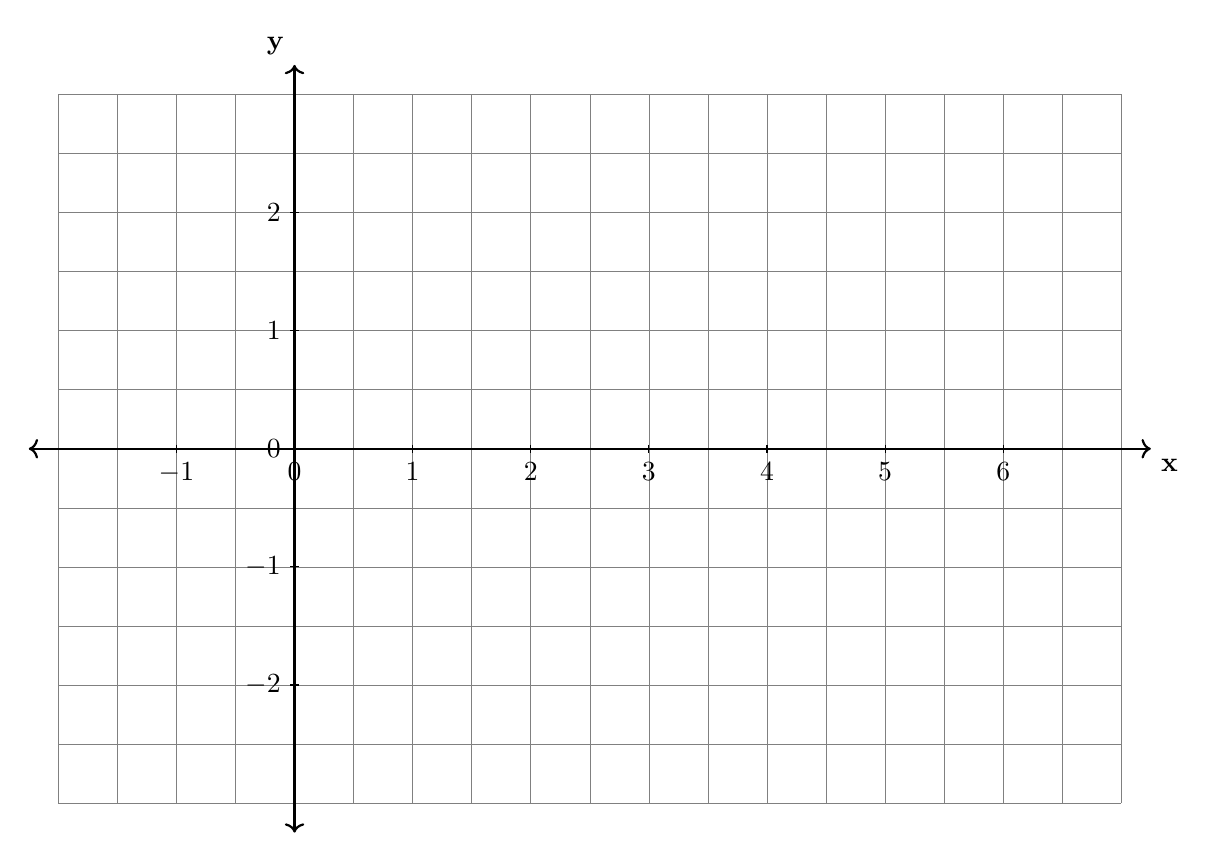
\begin{tikzpicture}[scale=6/4]
    \draw[step=0.5cm,gray,very thin] (-2,-3) grid (7,3);
    \draw[thick,<->] (-2.25,0) -- (7.25,0) node[anchor=north west] {\textbf{x}};
    \draw[thick,<->] (0,-3.25) -- (0,3.25) node[anchor=south east] {\textbf{y}};
    \foreach \x in {-1, 0, 1, 2, 3, 4, 5, 6} \draw (\x cm,1pt) -- (\x cm,-1pt) node[anchor=north] {$\x$};
    \foreach \y in {-2, -1, 0, 1, 2} \draw (1pt,\y cm) -- (-1pt,\y cm) node[anchor=east] {$\y$};
    %\foreach \y in {-5} \draw (1pt,\y cm) -- (-1pt,\y cm) node[anchor=east] {-50};    \tkzInit[xmin=-5,xmax=5,ymin=-7,ymax=7,ystep=1]   
%    \tkzFct[color=black,thick,<->,domain = -3.4:7] {0.1*(x*x-4)*(x-5)};
    \end{tikzpicture}
\end{center}

\newpage

\item Simplify the expression $(5 - 3i)^2$, where $i$ is the imaginary unit. \\*[1.25in]

\item Given $i$ is the imaginary unit, $(1-ai)^2$ in simplest form is what?  \\*[1.25in]%Alg2 Regents Jun2016


\item Write $\sqrt{x^4} \bullet \sqrt{x^3}$ as a single term with a rational exponent.\\*[1in]

\item When $b>0$ and $d$ is a positive integer, the expression $\displaystyle \left(8x^6 \right)^\frac{1}{3}$ is equivalent to what expressed as a radical? \\*[1in]%Alg2 Regents Jun2016 multiple choice

\item What does $\displaystyle \left( \frac{9x^3}{y^6} \right)^\frac{1}{2}$ equal?

\newpage
\item What is the inverse of $f(x)=-6(x-2)$? %Regents Alg2 Jan2018 multiple choice

Difficulty=6
\item What is the inverse of $\displaystyle f(x)=\frac{x+1}{x-2}$? %Alg2 Regents Aug2017 multiple choice

\item What are the zeros of the function $f(x)=x^3-5x^2-4x+20$? 

\item The graph of $y = f(x)$ is shown below. The function has a leading coefficient of 1.\\*
\begin{center}
    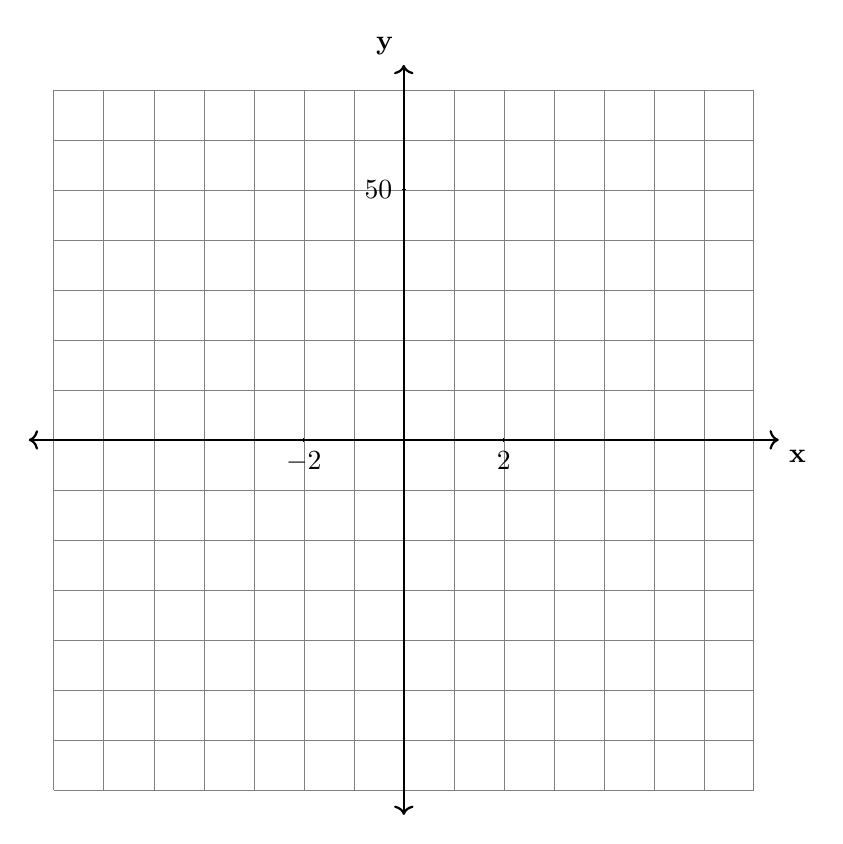
\begin{tikzpicture}[scale=2.54/4]
    \draw[step=1cm,gray,very thin] (-7,-7) grid (7,7);
    \draw[thick,<->] (-7.5,0) -- (7.5,0) node[anchor=north west] {\textbf{x}};
    \draw[thick,<->] (0,-7.5) -- (0,7.5) node[anchor=south east] {\textbf{y}};
    \foreach \x in {-2, 2} \draw (\x cm,1pt) -- (\x cm,-1pt) node[anchor=north] {$\x$};
    \foreach \y in {5} \draw (1pt,\y cm) -- (-1pt,\y cm) node[anchor=east] {50}; %{$\y$};
    \tkzInit[xmin=-5,xmax=5,ymin=-7,ymax=7,ystep=1]   
    \tkzFct[color=black,thick,<->,domain = -4.4:3.6] {0.1*(x+4)*x*x*(x-3)};
    \end{tikzpicture}
\end{center}
Write an equation for $f(x)$.\\*[10pt]
The function $g$ is formed by translating function $f$ left 2 units. Write an equation for $g(x)$.

\newpage
\item If the function $g(x) = ab^x$ represents exponential growth, which statement about $g(x)$ is false?
\begin{enumerate}
    \item $a > 0$ and $b>1$
    \item The $y$-intercept is $(0, a)$.
    \item The asymptote is $y=0$.
    \item The $x$-intercept is $(b,0)$
\end{enumerate} %Alg2 Regents Jan2018 multiple choice

\item A certain pain reliever is taken in 220 mg dosages and has a half-life of 12 hours. The function $\displaystyle A = 220 \left( \frac{1}{2} \right) ^\frac{t}{12}$ can be used to model this situation, where $A$ is the amount of pain reliever in milligrams remaining in the body after $t$ hours.\\*
According to this function, which statement is true?
\begin{enumerate}
    \item Every hour,the amount of pain reliever remaining is cut in half. 
    \item In 12 hours, there is no pain reliever remaining in the body.
    \item In 24 hours, there is no pain reliever remaining in the body.
    \item In 12 hours, 110 mg of pain reliever is remaining.
\end{enumerate}

\item Judith puts \$5000 into an investment account with interest compounded continuously. What is the approximate annual rate is needed for the account to grow to \$9110 after 30 years?

\end{enumerate}
\end{document}
